\documentclass[12pt,a4paper]{report}
% Layout shared by the coursework reports in this repository.
\usepackage{fontspec}
\IfFontExistsTF{DejaVu Sans Mono}{\setmonofont[Scale=0.84]{DejaVu Sans Mono}}{}
\usepackage[vietnamese]{babel}
\usepackage[a4paper,margin=1in]{geometry}
\usepackage{amsmath,amssymb,mathtools,bm}
\usepackage{booktabs,tabularx,array,longtable}
\usepackage{graphicx,float}
\usepackage{enumitem}
\usepackage{fancyhdr,setspace,titlesec,caption,microtype,needspace,etoolbox}
\usepackage[hidelinks]{hyperref}

\setstretch{1.15}
\setlength{\parskip}{0.45em}
\setlength{\parindent}{0pt}
\setlength{\headheight}{16pt}
\setcounter{tocdepth}{2}
\setcounter{secnumdepth}{3}
\emergencystretch=2em

\captionsetup{font=small,labelfont=bf}
\numberwithin{equation}{chapter}

\titleformat{\chapter}[display]
  {\normalfont\bfseries}
  {\filleft\Large\chaptertitlename\ \thechapter}
  {0.35em}
  {\filright\huge}
  [\vspace{0.4em}\titlerule]
\titlespacing*{\chapter}{0pt}{-10pt}{22pt}
\titleformat{\section}{\Large\bfseries}{\thesection}{0.6em}{}
\titleformat{\subsection}{\large\bfseries}{\thesubsection}{0.6em}{}
\titleformat{\subsubsection}{\normalsize\bfseries}{\thesubsubsection}{0.6em}{}

\preto\section{\Needspace{5\baselineskip}}{}
\preto\subsection{\Needspace{4\baselineskip}}{}
\preto\subsubsection{\Needspace{3\baselineskip}}{}

\newcommand{\CourseReportHeader}[1]{%
  \pagestyle{fancy}%
  \fancyhf{}%
  \fancyhead[L]{\small\nouppercase{\leftmark}}%
  \fancyhead[R]{\small #1}%
  \fancyfoot[C]{\thepage}%
  \fancypagestyle{plain}{%
    \fancyhf{}%
    \fancyhead[L]{\small\nouppercase{\leftmark}}%
    \fancyhead[R]{\small #1}%
    \fancyfoot[C]{\thepage}%
  }%
}

\newcommand{\R}{\mathbb{R}}
\newcommand{\norm}[1]{\left\lVert #1 \right\rVert}
\newcommand{\code}[1]{\texttt{\detokenize{#1}}}

% Arguments: logo, report type, course, title, author label, metadata rows, date.
\newcommand{\CourseCover}[7]{%
  \hypersetup{pageanchor=false}%
  \begin{titlepage}
    \centering
    \vspace*{0.5cm}
    {\normalsize\bfseries ĐẠI HỌC QUỐC GIA THÀNH PHỐ HỒ CHÍ MINH\par}
    {\normalsize\bfseries TRƯỜNG ĐẠI HỌC BÁCH KHOA\par}
    {\normalsize\bfseries KHOA KHOA HỌC VÀ KỸ THUẬT MÁY TÍNH\par}
    \vspace{0.6cm}
    \includegraphics[width=0.2\textwidth]{#1}\par
    \vspace{0.7cm}
    {\large\bfseries #2\par}
    \vspace{0.35cm}
    {\normalsize\textbf{#3}\par}
    {\small Học kỳ 261 · Năm học 2026–2027\par}
    \vspace{0.45cm}
    {\LARGE\bfseries #4\par}
    \vspace{0.6cm}
    {\normalsize\bfseries #5\par}
    \vspace{0.35cm}
    {\small\begin{tabular}{@{}ll@{}}#6\end{tabular}\par}
    \vfill
    {\small\bfseries Thành phố Hồ Chí Minh, #7\par}
  \end{titlepage}
  \pagenumbering{roman}%
  \hypersetup{pageanchor=true}%
}

\newcommand{\CourseFrontChapter}[1]{%
  \chapter*{#1}%
  \addcontentsline{toc}{chapter}{#1}%
  \markboth{#1}{#1}%
}

\newcommand{\CourseAbstract}[1]{%
  \CourseFrontChapter{Tóm tắt}%
  #1\par
}

\newcommand{\CourseOverview}[1]{%
  \CourseFrontChapter{Tổng quan báo cáo}%
  \begingroup
  \renewcommand{\arraystretch}{1.3}%
  \begin{tabularx}{\textwidth}{@{}>{\bfseries\raggedright\arraybackslash}p{3.3cm}>{\raggedright\arraybackslash}X@{}}
    #1
  \end{tabularx}
  \endgroup
}

% Omit the figure list for a report containing only tables.
\newcommand{\CourseContents}[1][\listoffigures]{%
  \tableofcontents
  #1%
  \listoftables
  \clearpage
  \pagenumbering{arabic}%
}

\CourseReportHeader{CO5085 · A1}
\newcommand{\resultfigure}[3]{\IfFileExists{notebook-evidence/figures/#1.png}{\begin{figure}[htbp]\centering\includegraphics[width=#3\textwidth]{notebook-evidence/figures/#1.png}\caption{#2}\end{figure}}{}}
\hypersetup{pdftitle={CO5085 - Bao cao A1},pdfauthor={Huynh Thanh Dat - 2570161}}

\begin{document}
\CourseCover{assets/hcmut-logo.png}
  {BÁO CÁO BÀI TẬP LỚN A1}
  {CO5085 · Học sâu và ứng dụng trong thị giác máy tính}
  {So sánh ResNet18 và Swin-T trên CIFAR-100}
  {Sinh viên}
  {Huỳnh Thành Đạt & 2570161\\[0.5em]
   Giảng viên & Lê Thành Sách\\
              & Nguyễn Quốc Minh}
  {tháng 11 năm 2026}

\CourseAbstract{
Thực nghiệm so sánh ResNet18 và Swin-T trên CIFAR-100 để khảo sát ảnh hưởng của tiền huấn luyện và số tầng được cập nhật. Thiết lập 20 epoch gồm tám cấu hình với ba hạt giống. Mỗi kiến trúc được huấn luyện từ đầu và thử ba chế độ với trọng số ImageNet, gồm chỉ học bộ phân loại, tinh chỉnh một phần và tinh chỉnh toàn bộ.

Trong thiết lập 20 epoch, Swin-T tinh chỉnh toàn bộ đạt độ chính xác cao hơn ResNet18 và cần nhiều thời gian, bộ nhớ hơn. Hai bản Swin-T chạy dưới cùng lịch 40 epoch đạt lần lượt 60,30\% khi khởi tạo ngẫu nhiên và 86,39\% khi dùng trọng số ImageNet. Độ chính xác của bản ngẫu nhiên tăng rõ so với cấu hình 20 epoch, trong đó quá trình học dừng gần mức đoán ngẫu nhiên ở một số lượt.
}

\CourseOverview{
Bài toán & Phân loại 100 lớp ảnh CIFAR-100.\\
Kiến trúc & ResNet18 và Swin-T. Các bản tiền huấn luyện dùng trọng số ImageNet.\\
Đối chứng & Huấn luyện từ đầu, chỉ học đầu ra, tinh chỉnh một phần và tinh chỉnh toàn bộ.\\
Phép đo & Độ chính xác, macro-F1, thời gian và bộ nhớ trong hai thiết lập với tổng cộng 30 lượt.\\
Kết quả chính & Swin-T từ đầu đạt 60,30\% trong lịch 40 epoch. Bản ImageNet cùng lịch đạt 86,39\%.\\
Giới hạn & Cách chia có một số ảnh trùng pixel. Phép đối chứng 40 epoch dành riêng cho Swin-T.\\
}

\CourseContents

\chapter{Bài toán và dữ liệu}
\section{Mục tiêu và phạm vi}
A1 so sánh CNN và Transformer trên CIFAR-100, tập trung vào ảnh hưởng của
khởi tạo pretrained và mức độ đóng băng backbone. Hai kiến trúc được chọn là
ResNet18 và Swin-T của torchvision. Thí nghiệm chính gồm 24 lượt, với bốn chế độ
huấn luyện cho mỗi kiến trúc và ba hạt giống 42, 43, 44. Thí nghiệm bổ sung
khảo sát riêng cách khởi tạo Swin-T dưới cùng lịch huấn luyện 40 epoch.

Các so sánh chính gồm huấn luyện từ đầu với pretrained, và head-only với
partial/full fine-tuning. Accuracy, macro-F1, thời gian và bộ nhớ được dùng
để đánh giá hiệu quả cùng chi phí của từng chế độ.

\section{CIFAR-100 và tình trạng license}
CIFAR-100 gồm 60.000 ảnh màu $32\times32$, 100 nhãn chi tiết (fine classes)
và 20 nhóm coarse classes. Bài này dự đoán toàn bộ 100 fine classes; không
chọn subset ảnh hoặc lớp. Mỗi lớp có 500 ảnh official train và 100 ảnh
official test \cite{cifar}. Số lớp lớn hơn bài E1 và ảnh độ phân giải thấp
có thể làm những lớp gần nhau khó phân biệt.

Nguồn chính là trang CIFAR của Toronto, của Alex Krizhevsky, Vinod Nair và
Geoffrey Hinton. Trang này không nêu license tường minh; thẻ dataset chính
thức \code{uoft-cs/cifar100} trên Hugging Face ghi \emph{license: unknown}
\cite{cifar,hf}. Vì vậy, tình trạng license của dữ liệu được ghi là chưa rõ.
Bản lưu CIFAR-100 dùng cho thực nghiệm được đối chiếu mã băm với bản gốc của Toronto. Dữ liệu ảnh được lưu riêng.

\section{Phân bố dữ liệu và cách chia tập}
Trong 50.000 ảnh phát triển, chỉ số được xáo theo từng lớp bằng hạt giống
2026. Mỗi lớp đóng góp 450 ảnh cho tập huấn luyện và 50 ảnh cho tập xác thực.
Tập kiểm tra chính thức gồm 100 ảnh mỗi lớp. Ba tập lần lượt có 45.000,
5.000 và 10.000 ảnh, nên sai khác về số ảnh giữa các lớp không chi phối
độ chính xác chung. Trung bình RGB của tập huấn luyện trên thang $[0,1]$
là $(0{,}507,0{,}487,0{,}441)$. Phép đối chiếu theo pixel phát hiện một số
ảnh lặp, được phân tích riêng ở phần giới hạn.

\section{Tiền xử lý và tải dữ liệu}
Ảnh huấn luyện được đệm bốn pixel, cắt ngẫu nhiên về $32\times32$ và lật
ngang với xác suất 0,5. Sau đó ảnh được nội suy song tuyến tính lên
$96\times96$. Tập xác thực và tập kiểm tra chỉ dùng bước nội suy.
Cả hai kiến trúc chuẩn hóa ảnh với trung bình ImageNet
$(0{,}485,0{,}456,0{,}406)$ và độ lệch chuẩn $(0{,}229,0{,}224,0{,}225)$.
DataLoader xáo thứ tự ảnh huấn luyện. Phép biến đổi của từng ảnh được
xác định theo hạt giống, epoch và chỉ số ảnh, để một lượt tiếp tục từ
checkpoint nhận lại đúng chuỗi biến đổi.

\chapter{Kiến trúc và chế độ huấn luyện}
\section{ResNet18: đối chứng CNN}
Giữ kiến trúc ResNet18 chuẩn torchvision, gồm stem convolution $7\times7$,
max pooling và bốn residual stages. Một residual block cập nhật
\begin{equation}
h_{l+1}=\operatorname{ReLU}\left(F_l(h_l)+S_l(h_l)\right),
\end{equation}
trong đó $S_l$ là identity hoặc projection khi đổi số kênh/stride. Kernel
convolution chia sẻ trọng số theo vị trí và khai thác quan hệ cục bộ. Sau
adaptive average pooling, head Linear được thay để dự đoán 100 lớp; không
thay stem thành biến thể ResNet chuyên cho CIFAR.

Bản pretrained dùng \code{ResNet18_Weights.IMAGENET1K_V1}. Ba chế độ là
chỉ học \code{fc}; học \code{layer4} và \code{fc}; học toàn bộ. Bản scratch
khởi tạo mới và học toàn bộ. BatchNorm trong phần frozen ở eval, nên cả
tham số lẫn running mean/variance và bộ đếm batch được giữ nguyên.

\section{Swin-T: đối chứng Transformer}
Swin-T dùng patch embedding stride4, các stage Transformer theo cấp độ và
patch merging. Attention trên cửa sổ có dạng
\begin{equation}
\operatorname{Attention}(Q,K,V)
=\operatorname{softmax}\left(\frac{QK^\top}{\sqrt{d}}+B+M\right)V,
\end{equation}
trong đó $B$ là relative position bias, $M$ là mask của shifted windows.
Dịch cửa sổ giúp trao đổi thông tin giữa cửa sổ qua các block; việc giới hạn
attention trong cửa sổ khác với global attention của ViT cổ điển.

Swin-T giữ kiến trúc chuẩn torchvision, với \code{head} được thay bằng
Linear 100 lớp. Đầu vào $96\times96$ tạo lưới patch đầu $24\times24$;
các stage muộn có lưới nhỏ hơn. Kích thước cửa sổ mặc định là 7, với padding
nội bộ ở những stage có kích thước không chia hết cho cửa sổ.

Bản pretrained dùng \code{Swin_T_Weights.IMAGENET1K_V1}. Chế độ partial chỉ
học stage cuối \code{features.7}, \code{norm} cuối và \code{head}; patch
merging đứng trước stage cuối vẫn frozen. Head-only chỉ học head. Frozen
stages được giữ ở eval, bao gồm stochastic depth, để đặc trưng của phần
đóng băng ổn định trong quá trình học head. Full và scratch cập nhật toàn bộ mô hình.

\section{Ma trận đối chứng}
\begin{table}[htbp]\centering
\begin{tabular}{lll}
\toprule
Chế độ & Khởi tạo backbone & Phần được cập nhật\\\midrule
Scratch & Ngẫu nhiên & Toàn bộ\\
Head-only & ImageNet pretrained & Head100\\
Partial & ImageNet pretrained & Stage cuối và head; Swin thêm norm\\
Full & ImageNet pretrained & Toàn bộ\\\bottomrule
\end{tabular}
\caption{Bốn chế độ cho mỗi họ kiến trúc, cùng split và ba seed.}
\end{table}
Scratch cập nhật toàn bộ mô hình từ khởi tạo ngẫu nhiên. Số tham số tổng và
trainable được đếm trực tiếp từ từng mô hình và lưu trong metadata.
ResNet18 và Swin-T khác nhau về kiến trúc, capacity và recipe pretrained;
các kết quả phản ánh tổng thể những khác biệt này trong cùng thiết lập.

\chapter{Thiết lập thực nghiệm và phép đo}
\section{Thiết lập 20 epoch}
Mỗi lượt của thí nghiệm chính có 20 epoch, batch 128 (giữ batch cuối), vòng lặp huấn luyện trực tiếp,
AdamW với weight decay $10^{-4}$, $\beta=(0{,}9,0{,}999)$, epsilon $10^{-8}$.
Learning rate ban đầu là $10^{-3}$ cho scratch/head và $10^{-4}$ cho
pretrained partial/full. Cosine scheduler bước một lần sau epoch:
\begin{equation}
\eta_e=\frac{\eta_0}{2}\left[1+\cos\left(\frac{\pi e}{20}\right)\right],
\end{equation}
với $e=0$ trước epoch đầu. Loss cross-entropy không label smoothing:
\begin{equation}
\mathcal{L}=-\frac1B\sum_{i=1}^{B}\log
\frac{\exp z_{i,y_i}}{\sum_{c=1}^{100}\exp z_{i,c}}.
\end{equation}
Clip global gradient norm ở 1 trước optimizer.step. BF16 autocast áp dụng
cho tất cả chế độ; tham số và Adam moments giữ FP32, không GradScaler,
TF32 tắt và không dùng compile. Các phép đo được thiết lập trên RTX 5090 với
tám worker tải dữ liệu và bốn luồng CPU.

Ngân sách 20 epoch được giữ cố định giữa các chế độ. Learning rate của
head/scratch và partial/full được đặt khác nhau để phù hợp với mức độ cập
nhật backbone. Kết quả vì vậy được phân tích theo từng thiết lập đầy đủ;
mức hội tụ còn được đối chiếu qua đường cong train/validation.

\section{Thiết lập 40 epoch cho Swin-T}

Trong lịch 20 epoch, hai lượt Swin-T khởi tạo ngẫu nhiên có độ chính xác xác thực
1\% ở epoch cuối và cross-entropy huấn luyện gần $\ln(100)$. Vì sai số cao
ngay trên tập huấn luyện, điểm thấp cho thấy quá trình tối ưu chưa học được
biểu diễn phân lớp trong thiết lập đó. So sánh trực tiếp với bản ImageNet
trong điều kiện này sẽ phóng đại chênh lệch giữa hai cách khởi tạo.

Thí nghiệm bổ sung giữ kiến trúc, cách chia tập, tiền xử lý, batch 128 và
ba hạt giống. Hai bản cập nhật toàn bộ tham số và chỉ khác nguồn trọng số
backbone. Cả hai dùng AdamW với hệ số suy giảm trọng số $10^{-2}$, tốc độ học
tăng tuyến tính từ $2\times10^{-5}$ đến $2\times10^{-4}$ qua năm epoch
làm nóng, rồi giảm theo cosine đến cuối lịch 40 epoch. Lịch tăng dần
và giảm cosine dựa trên cách huấn luyện Swin trong bài báo gốc \cite{swin},
với ngân sách và tốc độ học điều chỉnh cho CIFAR-100. Thay đổi đồng thời
lịch, ngân sách và hệ số suy giảm trọng số giúp kiểm tra cấu hình có học
ổn định hơn hay không. Phép so sánh giữa hai lịch không tách riêng đóng góp
của từng thay đổi.

\section{Chọn checkpoint và mở test}
Best chọn bằng val accuracy lớn nhất; hòa accuracy thì lấy CE nhỏ nhất,
hòa cả hai giữ epoch trước. Chỉ val được dùng ra quyết định trong train.
Test được đánh giá ở một bước riêng sau khi hoàn tất các lượt huấn luyện.
Các cấu hình, learning rate và seed được cố định trước bước này.

Accuracy và macroF1 đều tính trên 100 lớp. Với mỗi lớp $c$,
\begin{equation}
F1_c=\frac{2TP_c}{2TP_c+FP_c+FN_c},\qquad
F1_{macro}=\frac1{100}\sum_{c=1}^{100}F1_c.
\end{equation}
Trường hợp mẫu số bằng0 có F1 bằng0. Confusion matrix, support, precision,
recall, F1 theo lớp và từng prediction được lưu để kiểm tra. Gallery lấy tối
đa 8 lỗi confidence cao nhất của seed 42.

\section{Chi phí và môi trường}
Training time bao gồm data loading/augmentation và train pass, có CUDA
synchronize trước/sau. Epoch time thêm validation. Model construction,
checkpoint và report export nằm ngoài hai khoảng đo; không gọi training time
là tổng wall time của job. Peak GPU memory là peak allocated trong train và
validation của mỗi epoch, không phải reserved memory hoặc VRAM toàn hệ thống.

Metadata lưu GPU, torch/torchvision, CUDA/cuDNN, workers, CPU threads và
chế độ deterministic. Các phép đo thời gian của cùng cấu hình được gộp khi
những thông số môi trường này thống nhất.

\section{Thông tin tái lập}
Mỗi lượt lưu trạng thái huấn luyện ở cuối epoch để có thể tiếp tục từ mốc hoàn tất gần nhất. Checkpoint có kết quả xác thực tốt nhất giữ trọng số và chỉ số dùng để chọn mô hình. Dữ liệu, cách chia tập, mã nguồn và môi trường thực nghiệm được ghi nhận cùng từng lượt. Sai khác phần cứng hoặc thư viện có thể ảnh hưởng khả năng tái lập từng bit.

\href{https://github.com/dathuynh1108/CO5085-deep-learning/blob/main/notebooks/A1.ipynb}{Notebook A1}
trình bày từ khảo sát dữ liệu đến huấn luyện và đánh giá. Các tệp cấu hình và kết quả theo hạt giống
cho phép đối chiếu bảng với checkpoint đã chọn.

\chapter{Kết quả trong thiết lập 20 epoch}
\section{So sánh các chế độ huấn luyện}
\begin{table}[htbp]\centering\small
\setlength{\tabcolsep}{5pt}
\begin{tabular}{lrrr}
\toprule
Cấu hình & Validation (\%) & Test (\%) & Macro-F1 \\
\midrule
ResNet18 Scratch & 64{,}25 $\pm$ 0{,}18 & 64{,}53 $\pm$ 0{,}36 & 0{,}6441 $\pm$ 0{,}0032 \\
ResNet18 Head-only & 62{,}06 $\pm$ 0{,}12 & 60{,}89 $\pm$ 0{,}06 & 0{,}6076 $\pm$ 0{,}0008 \\
ResNet18 Partial & 74{,}04 $\pm$ 0{,}15 & 73{,}91 $\pm$ 0{,}18 & 0{,}7388 $\pm$ 0{,}0017 \\
ResNet18 Full & 78{,}87 $\pm$ 0{,}19 & 78{,}93 $\pm$ 0{,}10 & 0{,}7891 $\pm$ 0{,}0011 \\
Swin-T Scratch & 2{,}26 $\pm$ 1{,}49 & 2{,}19 $\pm$ 1{,}35 & 0{,}0067 $\pm$ 0{,}0075 \\
Swin-T Head-only & 72{,}37 $\pm$ 0{,}11 & 71{,}75 $\pm$ 0{,}05 & 0{,}7161 $\pm$ 0{,}0007 \\
Swin-T Partial & 78{,}69 $\pm$ 0{,}06 & 78{,}34 $\pm$ 0{,}26 & 0{,}7826 $\pm$ 0{,}0026 \\
Swin-T Full & 86{,}98 $\pm$ 0{,}11 & 86{,}54 $\pm$ 0{,}24 & 0{,}8653 $\pm$ 0{,}0025 \\
\bottomrule
\end{tabular}

\caption{Accuracy và macro-F1 của tám cấu hình, trung bình và SD mẫu qua ba seed. Accuracy theo phần trăm, F1 theo thang 0--1.}
\end{table}
Kết quả được tổng hợp bằng trung bình và độ lệch chuẩn mẫu qua các seed.
Danh sách lượt chạy và checkpoint tương ứng được lưu trong manifest.

\section{Thời gian, bộ nhớ và số tham số}
\begin{table}[htbp]\centering\small
\setlength{\tabcolsep}{4pt}
\begin{tabular}{llrrrr}
\toprule
Kiến trúc & Chế độ & Tổng (M) & Học (M) & Giây & MiB \\
\midrule
ResNet18 & Từ đầu & 11,228 & 11,228 & $86,6 \pm 5,4$ & $520,1 \pm 2,2$ \\
ResNet18 & Chỉ đầu ra & 11,228 & 0,051 & $80,1 \pm 0,2$ & $251,0 \pm 0,0$ \\
ResNet18 & Một phần & 11,228 & 8,445 & $80,2 \pm 0,2$ & $347,3 \pm 0,0$ \\
ResNet18 & Toàn bộ & 11,228 & 11,228 & $80,4 \pm 0,6$ & $518,9 \pm 0,0$ \\
Swin-T & Từ đầu & 27,596 & 27,596 & $211,1 \pm 1,6$ & $2451,8 \pm 0,2$ \\
Swin-T & Chỉ đầu ra & 27,596 & 0,077 & $86,1 \pm 0,5$ & $502,9 \pm 0,0$ \\
Swin-T & Một phần & 27,596 & 14,262 & $106,9 \pm 0,2$ & $667,7 \pm 0,0$ \\
Swin-T & Toàn bộ & 27,596 & 27,596 & $212,5 \pm 0,6$ & $2451,9 \pm 0,0$ \\
\bottomrule
\end{tabular}

\caption{Tổng tham số và tham số được học theo triệu (M), thời gian huấn luyện đủ 20 epoch và bộ nhớ cấp phát cực đại ở hạt giống 42 trên cùng máy.}
\end{table}

\section{Thảo luận kết quả}
\subsection{Ảnh hưởng của mức tinh chỉnh}

ResNet18 chỉ học bộ phân loại đạt 60,95\%, thấp hơn 64,35\% của bản học từ đầu. Khi các tầng đặc trưng giữ nguyên, bộ phân loại tuyến tính chỉ có thể thay đổi ranh giới trên biểu diễn đã học từ ImageNet. Tinh chỉnh khối cuối đạt 73,96\%, còn cập nhật toàn bộ đạt 78,97\%. Kết quả cho thấy mức thích nghi của bộ trích xuất đặc trưng có ảnh hưởng đáng kể trên CIFAR-100.

Swin-T chỉ học bộ phân loại đạt 71,67\%, tinh chỉnh một phần đạt 78,25\% và tinh chỉnh toàn bộ đạt 86,63\%. Bản khởi tạo ngẫu nhiên ở lịch 20 epoch chỉ đạt 2,76\%. Hai trong ba seed kết thúc ở 1\% trên tập validation, với cross-entropy huấn luyện gần $\ln(100)$. Điểm thấp xuất hiện trên cả hai tập, phù hợp với việc tối ưu chưa học được biểu diễn hữu ích. Lịch 40 epoch ở chương sau dùng chung tốc độ học và cách cập nhật cho hai cách khởi tạo Swin-T.

\subsection{Chi phí và lỗi phân loại}

Khi tinh chỉnh toàn bộ, Swin-T cao hơn ResNet18 7,66 điểm phần trăm độ chính xác trên tập test. Tính theo trung bình ba seed, Swin-T cần thời gian huấn luyện gấp 2,64 lần và bộ nhớ cấp phát cực đại gấp 4,73 lần. Với Swin-T, chỉ học bộ phân loại hoặc tinh chỉnh khối cuối giảm thời gian và bộ nhớ so với cập nhật toàn bộ, nhưng độ chính xác cũng thấp hơn. Với ResNet18, thời gian của ba chế độ tiền huấn luyện gần nhau trong lần đo này, trong khi bộ nhớ giảm rõ khi đóng băng nhiều tầng hơn.

Ở epoch 20, ResNet18 tinh chỉnh toàn bộ đạt khoảng 99,1\% trên tập huấn luyện và 79,2\% trên tập validation; Swin-T tương ứng đạt 98,7\% và 86,7\%. Khoảng cách này cho thấy sai số khái quát hóa vẫn còn dù độ chính xác huấn luyện cao. Checkpoint dùng để đánh giá được chọn theo độ chính xác trên tập validation. Trong cả hai ma trận của seed 42, lớp cây sồi thường bị gán thành cây phong. Các ví dụ sai cho thấy độ phân giải gốc $32\times32$ khiến chi tiết hình dáng và kết cấu khó phân biệt.


\section{Đường cong và lỗi phân loại}
Các hình dùng seed 42 đã định trước, không chọn seed theo kết quả test.
Ma trận lỗi dùng chỉ số lớp 0--99; danh sách tên lớp và số đếm đầy đủ nằm
trong các tệp CSV kèm báo cáo.
\resultfigure{resnet18_scratch_curves}{ResNet18 scratch: train/val CE và accuracy ở seed 42.}{0.95}
\resultfigure{swin_t_scratch_curves}{Swin-T scratch: train/val CE và accuracy ở seed 42.}{0.95}
\resultfigure{resnet18_full_curves}{ResNet18 pretrained full: đường cong ở seed 42.}{0.95}
\resultfigure{swin_t_full_curves}{Swin-T pretrained full: đường cong ở seed 42.}{0.95}
\resultfigure{resnet18_full_confusion_test}{Confusion matrix test của ResNet18 full ở seed 42; hàng là nhãn thực tế.}{0.9}
\resultfigure{swin_t_full_confusion_test}{Confusion matrix test của Swin-T full ở seed 42.}{0.9}
\resultfigure{resnet18_full_errors_test}{Các dự đoán sai có confidence cao của ResNet18 full ở seed 42, hiển thị ảnh gốc $32\times32$.}{0.95}
\resultfigure{swin_t_full_errors_test}{Các dự đoán sai có confidence cao của Swin-T full ở seed 42.}{0.95}

\chapter{Kết quả đối chứng khởi tạo Swin-T}
\begin{table}[htbp]
\centering\small
\setlength{\tabcolsep}{4pt}
\begin{tabular}{lrrr}
\toprule
Cấu hình & Validation (\%) & Test (\%) & Macro-F1 \\
\midrule
Swin-T Scratch & 60{,}23 $\pm$ 0{,}28 & 60{,}00 $\pm$ 0{,}47 & 0{,}5990 $\pm$ 0{,}0049 \\
Swin-T Full & 86{,}13 $\pm$ 0{,}12 & 86{,}45 $\pm$ 0{,}19 & 0{,}8644 $\pm$ 0{,}0020 \\
\bottomrule
\end{tabular}

\caption{Swin-T dưới cùng lịch 40 epoch, trung bình và độ lệch chuẩn mẫu qua ba hạt giống.}
\label{tab:swin-followup}
\end{table}

Với lịch 40 epoch, Swin-T scratch đạt accuracy test $60{,}00 \pm 0{,}47$\%, cao hơn rõ rệt so với 2,19\% của lịch 20 epoch. Đường cong train và validation đều cải thiện, cho thấy mô hình đã học được cách phân biệt các lớp. Tuy vậy, accuracy cuối lịch trên train gần 90\%, còn validation khoảng 60\%: khớp dữ liệu train vẫn dễ hơn phân loại ảnh mới. Các checkpoint scratch tốt nhất được chọn trong khoảng epoch 36--37.

Swin-T pretrained đạt $86{,}45 \pm 0{,}19$\% dưới cùng lịch. Để so sánh, lấy accuracy của bản pretrained trừ bản scratch ở từng seed, rồi tính trung bình ba chênh lệch. Kết quả là $26{,}45 \pm 0{,}40$ điểm phần trăm; bản pretrained cao hơn ở cả ba cặp. Như vậy, ngay khi bản scratch đã học được, khởi tạo từ ImageNet vẫn đem lại lợi ích lớn. Hai bản có cùng kiến trúc, cập nhật toàn bộ tham số và dùng cùng lịch, nên phép so sánh này rõ hơn về vai trò của khởi tạo so với lịch 20 epoch.

\begin{table}[htbp]\centering\small
\setlength{\tabcolsep}{4pt}
\begin{tabular}{llrrrr}
\toprule
Kiến trúc & Chế độ & Tổng (M) & Học (M) & Giây & MiB \\
\midrule
Swin-T & Scratch & 27{,}596 & 27{,}596 & 428{,}1 $\pm$ 1{,}6 & 2453{,}2 $\pm$ 3{,}7 \\
Swin-T & Full & 27{,}596 & 27{,}596 & 429{,}7 $\pm$ 0{,}8 & 2456{,}7 $\pm$ 2{,}2 \\
\bottomrule
\end{tabular}

\caption{Chi phí lịch 40 epoch; thời gian train và peak allocated memory là trung bình và SD mẫu qua ba seed.}
\end{table}

Chi phí hai bản gần nhau: thời gian train đều khoảng 429 giây và bộ nhớ cấp phát cực đại khoảng 2455 MiB. Khác biệt chính trong đối chứng này nằm ở chất lượng phân loại, không phải số tham số hoặc ngân sách tính toán.


\begin{figure}[htbp]
\centering
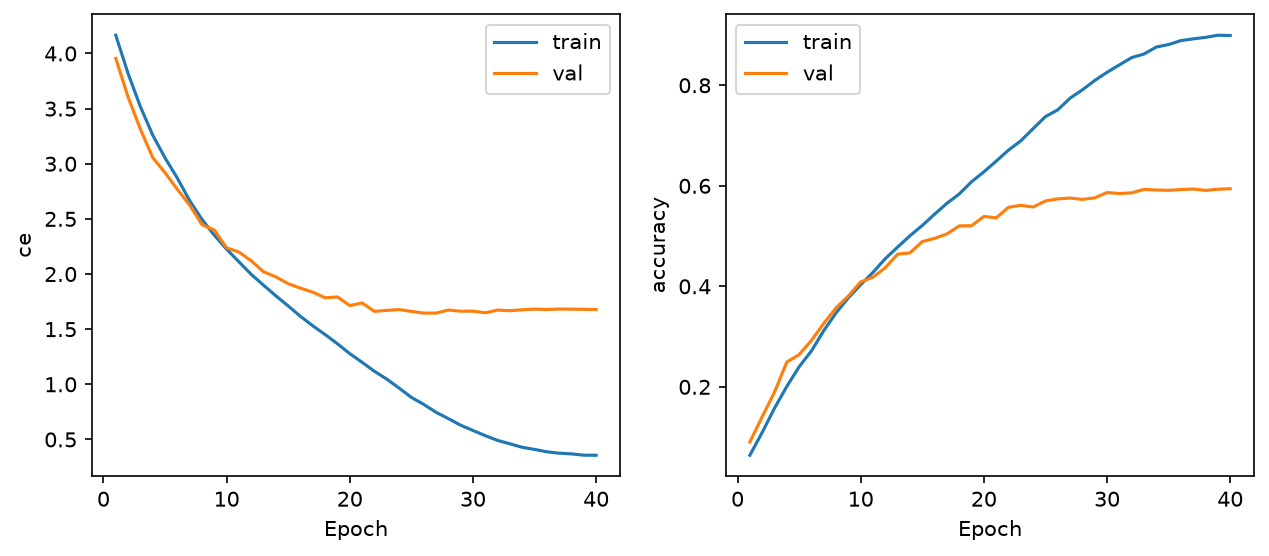
\includegraphics[width=0.94\linewidth]{swin-followup/figures/swin_t_scratch_curves.png}
\caption{Đường cong học của Swin-T khởi tạo ngẫu nhiên trong lịch 40 epoch, hạt giống 42.}
\end{figure}

\chapter{Kết luận và giới hạn}
\section{Kết luận}
Trong thiết lập 20 epoch, tinh chỉnh khối cuối hoặc toàn bộ cho độ chính xác cao hơn chỉ học bộ phân loại ở cả ResNet18 và Swin-T. Khi tinh chỉnh toàn bộ, Swin-T đạt độ chính xác cao hơn ResNet18 với chi phí huấn luyện và bộ nhớ lớn hơn. Đối chứng ở Bảng~\ref{tab:swin-followup} cho thấy cấu hình Swin-T khởi tạo ngẫu nhiên học được khi dùng lịch 40 epoch. Khoảng cách với bản ImageNet cần được đọc trong cùng lịch và trên cùng cách chia dữ liệu.

\section{Giới hạn}
Ảnh gốc $32\times32$ và đầu vào $96\times96$ khác với kích thước phổ biến
$224\times224$ của các bản tiền huấn luyện. Thực nghiệm khảo sát hai kiến
trúc trên CIFAR-100. Đối chứng bổ sung dành riêng cho Swin-T, nên không dùng để
xếp hạng hai kiến trúc dưới cùng lịch 40 epoch. Hai họ cũng khác số tham số
và quá trình tiền huấn luyện ImageNet.
Ba seed mô tả biến thiên giữa các lượt khởi tạo, với cùng phần cứng và
thiết lập workers. Tình trạng license của dữ liệu vẫn là chưa rõ.

\subsection{Ảnh trùng giữa các split}
Đối chiếu toàn bộ ảnh theo giá trị pixel phát hiện hai ảnh xác thực và mười ảnh kiểm tra trùng với ảnh huấn luyện. Các bảng sử dụng đủ 10.000 ảnh kiểm tra chính thức và giữ nguyên checkpoint đã chọn. Do mười ảnh trong số này đã xuất hiện khi huấn luyện, tập kiểm tra có một phần nội dung trùng với tập huấn luyện.

Tính lại trên 9.990 dự đoán sau khi loại mười ảnh trùng cho độ chính xác trung bình 79,009\% với ResNet18 và 86,677\% với Swin-T khi tinh chỉnh toàn bộ. Thứ hạng của hai cấu hình giữ nguyên. Phép kiểm tra độ nhạy dùng lại các dự đoán đã lưu. Hai ảnh xác thực trùng vẫn có thể ảnh hưởng việc chọn checkpoint, và phạm vi đối chiếu chỉ bao gồm các ảnh trùng pixel chính xác. Dữ liệu đối chiếu được lưu trong \code{docs/training-evidence/}.

Phạm vi hỗ trợ của AI được trình bày trong \href{https://github.com/dathuynh1108/CO5085-deep-learning/blob/main/AI\_USE\_REPORT.md}{\code{AI_USE_REPORT.md}}.

\begin{thebibliography}{9}
\addcontentsline{toc}{chapter}{Tài liệu tham khảo}
\bibitem{assignment} Lê Thành Sách, Nguyễn Quốc Minh. \emph{Bài tập lớn A1: CNN vs Transformer trên tập ảnh lớn}. CO5085, học kỳ 261.
\bibitem{cifar} A. Krizhevsky. \emph{Learning Multiple Layers of Features from Tiny Images}. 2009. Trang dataset: \url{https://www.cs.toronto.edu/~kriz/cifar.html}.
\bibitem{hf} uoft-cs. \emph{CIFAR100 dataset card}; license: unknown. \url{https://huggingface.co/datasets/uoft-cs/cifar100}.
\bibitem{resnet} K. He và cộng sự. \emph{Deep Residual Learning for Image Recognition}. CVPR 2016. \url{https://arxiv.org/abs/1512.03385}.
\bibitem{swin} Z. Liu và cộng sự. \emph{Swin Transformer: Hierarchical Vision Transformer using Shifted Windows}. ICCV 2021. \url{https://arxiv.org/abs/2103.14030}.
\bibitem{torchvision} Torchvision. ResNet18 và Swin-T model API; sử dụng weight enum IMAGENET1K\_V1. \url{https://docs.pytorch.org/vision/stable/models.html}.
\end{thebibliography}
\end{document}
